\documentclass[12pt,a4paper]{article}
\usepackage[affil-it]{authblk}
\usepackage{amsthm}
\usepackage{amssymb}
\usepackage{amsmath}
\usepackage{listings}
\usepackage{graphicx}
\usepackage{pgfplots}
\usepackage{float}
\usepackage{xcolor}
\usepackage{hyperref}
\usepackage[nameinlink]{cleveref}
\usepackage[Algorithm]{algorithm}
\usepackage{algpseudocode}

\usepackage[
  backend=bibtex,
  style=alphabetic,
  sorting=anyt,
  minnames=3,
  minalphanames=3
]{biblatex}

\hypersetup{
    colorlinks=true,
    citecolor=blue,
    linkcolor=black,
    urlcolor=blue,
    pdftitle={Approximation of Lambda-coloring in graphs},
}

\newtheorem{definition}{Definition}
\newtheorem{problem}{Problem}
\newtheorem{claim}{Claim}
\newtheorem{lemma}{Lemma}
\newtheorem{theorem}{Theorem}
\newtheorem{corollary}{Corollary}

\definecolor{sapRed}{HTML}{6f0a19}
\definecolor{sapBlue}{HTML}{006778}

\newcommand{\curlyquotes}[1]{\textquotedblleft #1\textquotedblright}
\newcommand{\abs}[1]{\left|#1\right|}
\newcommand{\abk}[1]{\left\langle#1\right\rangle}
\DeclareMathOperator{\dist}{dist}

\addbibresource{./references.bib}

\begin{document}

    \title{Approximations for $\lambda$-coloring in treewidth $k$ graphs, outerplanar graphs and split graphs}
    \author{Simone Bianco}
    \affil{Sapienza Università di Roma, Italy}
    \date{\today}

    \maketitle

    \abstract{This essay is based on the article written by \textcite{main_article}. The contents of in the article are discussed in a more in-depth way, showing graphical examples and providing access to a non-expert reader.}

    \tableofcontents
    \newpage

	\hypersetup{linkcolor=blue}

    \section{Introduction}

    
    In the context of radio frequency assignment, the goal is to allocate radio frequencies to transmitters at various locations while avoiding interference. This problem is analogous to graph coloring, where the vertices of the graph represent the transmitters, and the edges indicate potential interferences between adjacent vertices. The radio frequencies are represented as non-negative integers, often referred to as \curlyquotes{colors}.
    
    To model this problem, \textcite{L21_color} introduced the \textbf{$\mathbf{L(2, 1)}$-labeling problem}, where the transmitters are modeled as nodes of a graph whose edges depend on the capability of communication between the transmitters. The problem involves assigning colors to nodes under specific constraints:
    \begin{enumerate}
        \item Nodes that are very close to each other (at a distance of 1) must have a color value differing by at least two.
        \item Nodes that are relatively close (at a distance of 2) must have a color value differing by at least one.
    \end{enumerate}

    The problem is thus equivalent to defining an assignment, known as \textbf{$\lambda$-coloring}, from to each node in the network to integers from the set $\{0, \dots, \lambda\}$, known as the \textit{span}, ensuring the two constraints are satisfied. The objective of $\lambda$-coloring is to find the optimal (or near-optimal) bounds of the minimal value $\lambda_{2,1}$ that gives a span capable of coloring a graph. Over the years, the problem has been generalized to the $L(p,q)$-coloring, where $a$ and $b$ are two arbitrary non-negative integers.
    
    In this essay, we'll focus on the most studied values for this problem: $\lambda_{2,1}, \lambda_{1,1}$ and $\lambda_{0,1}$. In particular, we'll focus on studying bounds for these colorings on \textbf{graph classes}, i.e. sets of graphs with a given property.

    \begin{definition}
      Let $G$ be a graph and $p,q$ be two non-negative integers. A $\lambda$-coloring on $G$ is a function $f : V(G) \to \{0, \ldots , \lambda\}$. The $\lambda$-coloring satisfies the $L(p, q)$-constraints if
      \begin{itemize}
        \item For each $u,v \in V(G)$ such that $\dist(u,v) = 1$ it holds that $\abs{f(u) - f(v)} \geq p$
        \item For each $u,v \in V(G)$ such that $\dist(u,v) = 2$ it holds that $\abs{f(u) - f(v)} \geq q$
      \end{itemize}
      The minimum value $\lambda$ for which $G$ admits a $\lambda$-coloring satisfying the $L(p,q)$-constraint is denoted by $\lambda_{p,q}(G)$.
    \end{definition}

    The usual parameter used in these bounds is $\Delta$, i.e. the maximum degree of any node in the graph. For any general graph, the easiest lower bounds can be obtained from the tree graph $K_{1,\Delta}$, consisting of a tree with one root that has $\Delta$ children. Since any graph with maximum degree $\Delta$ contains $K_{1,\Delta}$ as a subgraph, the following lower bounds valid for any graph \cite{L21_color,lower_L01}:
    \[\lambda_{2,1} \geq \Delta+1 \qquad\qquad \lambda_{1,1} \geq \Delta \qquad\qquad \lambda_{0,1} \geq \Delta-1\]

    \cite{L21_color} also proved the general upper bound $\lambda_{2,1} \leq \Delta^2+2\Delta$, which was later improved to $\lambda_{2,1} \leq \Delta^2+\Delta$ in \cite{upper_L21}.

    For some special classes of graphs, tight bounds for $\lambda(\mathcal{G})$ are known and can be computed efficiently. Here, new upper bounds are provided for graphs of treewidth $k$, outerplanar graphs and split graphs.

    \section{Graphs of treewidth $k$}

    In graph theory, the \textit{treewidth} of an undirected graph is an integer number which specifies, informally, \curlyquotes{how far} the graph is from being a \curlyquotes{tree}. The treewidth is defined in terms of \textit{tree decomposition}.

    \begin{definition}
      A tree decomposition of a graph $G$ is a tree $T$ with nodes $V(T) = \{X_1, \ldots, X_t\}$ where $X_i \subseteq V(G)$ for any $i$ that satisfies the following properties:
      \begin{enumerate}
        \item The set $X_1, \ldots, X_t$ is a cover of $V$, meaning that each graph node is contained in at least one tree node.
        \item If $v \in X_i \cap X_j$ then all the tree nodes $X_h$ in the path from $X_i$ to $X_j$ contain $v$ as well.
        \item For all graph edge $(u,v)$, there is a subset $X_i$ that contains $v,w$
      \end{enumerate}
    \end{definition}

    The \textit{width} of a tree decomposition is the size of its largest set $X_i$ minus one. The \textit{treewidth} of a graph $G$, written as $\mathrm{tw}(G)$, is the minimum width among all possible tree decompositions of $G$. In this context, the minus one factor in the width measure is considered in order to make any standard tree have treewidth 1.

    \begin{figure}[H]
		\centering

		\begin{tabular}{ccc}
			\begin{tabular}{c}
				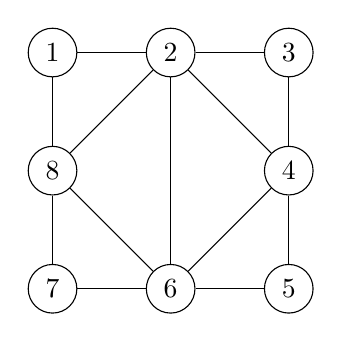
\begin{tikzpicture}[node distance=1.5cm]
					\node[circle, draw] (1)[] {$1$};
					\node[circle, draw] (2)[right of = 1] {$2$};
					\node[circle, draw] (3)[right of = 2] {$3$};
					\node[circle, draw] (4)[below of = 3] {$4$};
					\node[circle, draw] (5)[below of = 4] {$5$};
					\node[circle, draw] (6)[left of = 5] {$6$};
					\node[circle, draw] (7)[left of = 6] {$7$};
					\node[circle, draw] (8)[above of = 7] {$8$};

					\path[every node/.style={font=\sffamily\small}]
					(1) edge (2)
					(2) edge (3)
					(3) edge (4)
					(4) edge (5)
					(5) edge (6)
					(6) edge (7)
					(7) edge (8)
					(8) edge (1)

					(2) edge (4)
					(4) edge (6)
					(6) edge (8)
					(8) edge (2)

					(2) edge (6)
					;
				\end{tikzpicture}
			\end{tabular}

			&\qquad\qquad&

			\begin{tabular}{c}
				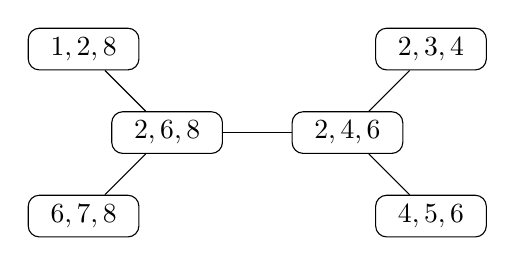
\begin{tikzpicture}[node distance=1.5cm]
					\node[rectangle, rounded corners, draw, minimum width=40] (1)[] {$1,2,8$};
					\node[rectangle, rounded corners, draw, minimum width=40] (2)[below right of = 1] {$2,6,8$};
					\node[rectangle, rounded corners, draw, minimum width=40] (3)[below left of = 2] {$6,7,8$};
					\node[rectangle, rounded corners, draw, minimum width=40] (4)[right of = 2, xshift = 22.5] {$2,4,6$};
					\node[rectangle, rounded corners, draw, minimum width=40] (5)[above right of = 4] {$2,3,4$};
					\node[rectangle, rounded corners, draw, minimum width=40] (6)[below right of = 4] {$4,5,6$};

					\path[every node/.style={font=\sffamily\small}]

						(1) edge (2)
						(2) edge (3)
						(2) edge (4)
						(4) edge (5)
						(4) edge (6)
					;
				\end{tikzpicture}
			\end{tabular}
		\end{tabular}
		\label{treewidth_2}
		\caption{A graph of treewidth 2 and his minimum width tree decomposition.}
    \end{figure}

	Through this definition, finding the treewidth of a graph is no easy task. An easier way to find the treewidth of a graph is through \textit{$k$-trees}, a generalization of the concept of standard trees. This class of graphs is inductively defined as follows.

	\begin{definition}
		Given an integer $k > 0$, a graph $G$ with $n$ nodes is said to be a $k$-tree if one of the two conditions holds: 
		\begin{itemize}
			\item $G$ is the complete graph $K_{k+1}$
			\item $G$ can be built from a $k$-tree $G'$ with $n-1$ nodes by adding a new node and making it adjacent to exactly all the vertices of a $k$-clique in $G'$
		\end{itemize}

		Any graph $H$ that is a subgraph of a $k$-tree is called a partial $k$-tree. 
	\end{definition}
	
	We notice that $k$-trees are exactly the maximal graphs with a treewidth of $k$ -- hence their name -- where \curlyquotes{maximal} means that no more edges can be added without increasing their treewidth. In fact, it can be shown that a graph is a partial $k$-tree if and only if its treewidth is at most $k$ \cite{k_trees_treewidth}. To show this result, we first state the following trivial lemma.

	\begin{theorem}{}
		A graph $G$ is a partial $k$-tree if and only if $\mathrm{tw}(G) \leq k$
	\end{theorem}

	\begin{proof}
		$\Rightarrow)$ Let $G = (V,E)$ be a partial $k$-tree and let $H = (V,E')$ be the $k$-tree that contains $G$ as a subgraph. Clearly, we have that $\mathrm{tw}(G) \leq \mathrm{tw}(H)$. We will show that $\mathrm{tw}(H) \leq k$. We proceed by induction on the number of vertices of $H$.
		
		If $H$ has $k+1$ vertices then $\mathrm{tw}(H) = k$ since a single node with all the vertices is a tree decomposition of $H$ of width $k$. Assume now that $H$ has more than $k+1$ vertices. By definition of $k$-tree, there is a node $v \in V$ such that $H[V-\{v\}$ is a $k$-tree and $v \cup N_H(v)$ induce a $(k+1)$-clique $K$ in $H$. By inductive hypothesis, the induced subgraph $H[V-\{v\}]$ has a tree decomposition $T = (\{X_1, \ldots, X_t\},F)$ of width at most $k$.
		
		Since $K-\{v\}$ is a $k$ clique in $H[V-\{v\}]$, by the previous lemma there must be a set $X_i$ such that $K-\{v\} \subseteq X_i$. Let $X_{t+1} = K$ and let $T' = (\{X_1, \ldots, X_t, X_{t+1}\}, F \cup \{i,t+1\})$. Then, since $\abs{K}-1 = k$, $T'$ is a tree decomposition of $G$ with width at most $k$.

		$\Leftarrow)$ Again, we proceed by induction. Let $G = (V,E)$. If $G$ has $k+1$ vertices then the $k$-tree $K_{k+1}$ trivially contains $G$.
		
		Assume now that now that $G$ has more than $k+1$ vertices. Let $T = (\{X_1, \ldots, X_t\},F)$ be a tree decomposition of $G$ of width at most $k$. Let $X_\ell$ be a leaf node of $T$ and let $X_i$ be its only neighbor in $T$. We can assume that $X_\ell \not\subseteq X_i$ since otherwise by removing $X_\ell$ from $T$ we still get a tree decomposition of $G$ with width at most $k$. Moreover, this assumption also allows us to assume that $X_\ell - X_i = \{v\}$: if not, $X_\ell$ can be divided into several tree nodes such that the resulting new leaf node satisfies this requirement.

		Since $X_\ell$ is a leaf node and $X_\ell - X_i = \{v\}$, every adjacent vertex of $v$ must be inside $X_\ell$ and $X_i$. Moreover, since $\abs{X_\ell} \leq k+1$, $v$ has at most $k$ such neighbors. By inductive hypothesis, $G[V-\{v\}]$ is a partial $k$ tree. Let $H$ be the $k$-tree that contains $G[V-\{v\}]$. By construction of $H$, $X_i$ must be a $k$-clique, hence by adding $v$ to $H$ and by connecting it to all the vertices in $X_i$, we get a $k$-tree that contains $G$.
	\end{proof}

	\begin{corollary}
		A graph $G$ has treewidth $k$ if and only if $k$ is the smallest value for which $G$ is a partial $k$-tree.
	\end{corollary}

	For instance, since in \Cref{treewidth_2} we have a graph of treewidth $2$, we know that it must be a partial $2$-tree, meaning that we can construct a $2$-tree that contains it. In fact, this graph is actually a full $2$-tree and not only a partial one.

    \begin{figure}[H]
		\centering

		\begin{tabular}{ccccc}
			\begin{tabular}{c}
				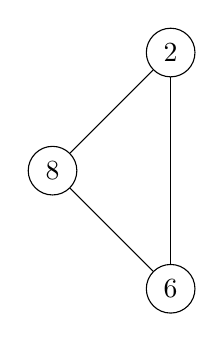
\begin{tikzpicture}[node distance=1.5cm]
					\node[] (1)[] {};
					\node[circle, draw] (2)[right of = 1] {$2$};
					\node[circle, draw] (8)[below of = 1] {$8$};
					\node[] (x)[below of = 8] {};
					\node[circle, draw] (6)[right of = x] {$6$};

					\path[every node/.style={font=\sffamily\small}]
					(2) edge (8)
					(8) edge (6)
					(6) edge (2)
					;
				\end{tikzpicture}
			\end{tabular}

			&\qquad&

			\begin{tabular}{c}
				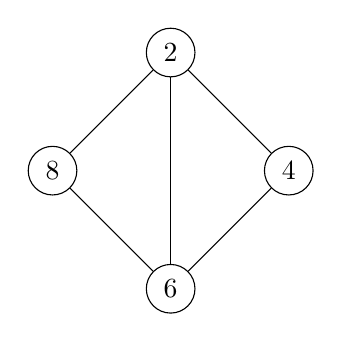
\begin{tikzpicture}[node distance=1.5cm]
					\node[] (1)[] {};
					\node[circle, draw] (2)[right of = 1] {$2$};
					\node[circle, draw] (8)[below of = 1] {$8$};
					\node[] (x)[below of = 8] {};
					\node[circle, draw] (6)[right of = x] {$6$};
					\node[] (y)[right of = 6] {};
					\node[circle, draw] (4)[above of = y] {$4$};


					\path[every node/.style={font=\sffamily\small}]
					(2) edge (8)
					(8) edge (6)
					(6) edge (2)
					(4) edge (2)
					(4) edge (6)
					;
				\end{tikzpicture}
			\end{tabular}

			&\qquad&

			\begin{tabular}{c}
				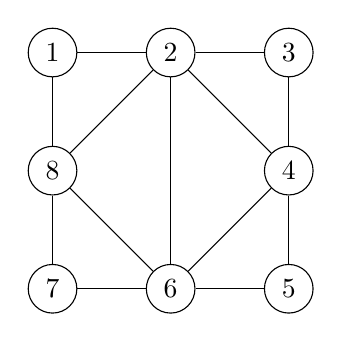
\begin{tikzpicture}[node distance=1.5cm]
					\node[circle, draw] (1)[] {$1$};
					\node[circle, draw] (2)[right of = 1] {$2$};
					\node[circle, draw] (3)[right of = 2] {$3$};
					\node[circle, draw] (4)[below of = 3] {$4$};
					\node[circle, draw] (5)[below of = 4] {$5$};
					\node[circle, draw] (6)[left of = 5] {$6$};
					\node[circle, draw] (7)[left of = 6] {$7$};
					\node[circle, draw] (8)[above of = 7] {$8$};

					\path[every node/.style={font=\sffamily\small}]
					(1) edge (2)
					(2) edge (3)
					(3) edge (4)
					(4) edge (5)
					(5) edge (6)
					(6) edge (7)
					(7) edge (8)
					(8) edge (1)

					(2) edge (4)
					(4) edge (6)
					(6) edge (8)
					(8) edge (2)

					(2) edge (6)
					;
				\end{tikzpicture}
			\end{tabular}
		\end{tabular}
		\caption{Steps 1, 2 and 6 of the inductive creation of the $2$-tree in \Cref{treewidth_2}}
    \end{figure}

	We observe that $k$-trees are also exactly the \textit{chordal graphs} whose maximal cliques all have size $k+1$ and whose minimal clique separators all have size $k$ \cite{k_trees_chordal}. A clique separator is a set of vertices in a graph that, when removed, disconnects the graph into multiple components, while the separator itself forms a clique.

	\begin{definition}
		A chordal graph is a graph in which all cycles of four or more vertices have a chord, i.e. an edge that is not part of the cycle but connects two vertices of the cycle.
	\end{definition}

	Equivalently, a chordal graph can be defined as a graph in which every induced cycle in the graph has exactly three vertices. For this reason, chordal graphs are also called \textit{triangulated graphs} -- again, see \Cref{treewidth_2}. Chordal graphs have a very special property: they always contain a perfect elimination sequence \cite{ordering}.

	\begin{lemma}
		A graph is chordal if and only if it contains a perfect elimination sequence.
	\end{lemma}

	A \textit{perfect elimination sequence} in a graph is an ordering of the vertices of the graph such that for all nodes $v$ it holds that $v$ and the neighbors of $v$ that occur after $v$ in the order form a clique.
	
	Since $k$-trees are a special type of chordal graph, any $k$-tree has a perfect elimination sequence. For instance, the ordering  $(1,3,5,7,4,2,8,6)$ is a perfect elimination sequence for the graph in \Cref{treewidth_2}.

	Using the fact that any graph with treewidth $k$ is a partial $k$-tree and that any $k$-tree is a chordal graph, we can define the following algorithm able to $\lambda$-color that satisfies the $L(p,q)$-constraints for any graph of treewidth $k$.

	\begin{figure}[H]
		\begin{algorithmic}[1]
			\Function{algorithm 1}{$G$, $\lambda, p,q$}
				\State Construct a $k$-tree $H$ that contains $G$ as a subgraph
				\State Construct a perfect elimination sequence $(v_1, \ldots, v_n)$ on $H$
				\For{$i$ = $n, \ldots, 1$}
					\State{Color $v_i$ with the smallest available color in $\{0,\ldots, \lambda\}$ \\satisfying the $L(p,q)$-coloring constraints in $G$}
				\EndFor
			\EndFunction
		\end{algorithmic}

		\caption{Algorithm for $\lambda$-Coloring Graphs of Treewidth $k$}
	\end{figure}

	\newpage

	To understand how the algorithm works, consider the following graph with treewidth 3.

    \begin{figure}[H]
		\centering

		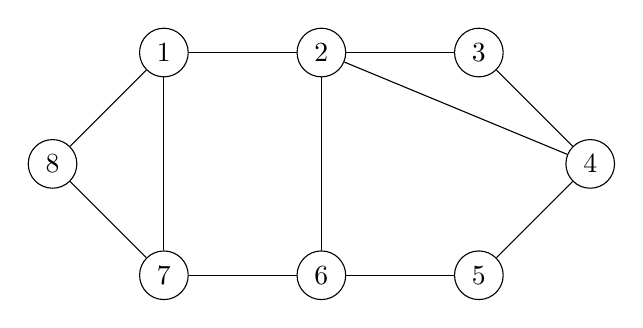
\begin{tikzpicture}[node distance=2cm]
			\node[circle, draw] (1)[] {$1$};
			\node[circle, draw] (2)[right of = 1] {$2$};
			\node[circle, draw] (3)[right of = 2] {$3$};
			\node[circle, draw] (4)[below right of = 3] {$4$};
			\node[circle, draw] (5)[below left of = 4] {$5$};
			\node[circle, draw] (6)[left of = 5] {$6$};
			\node[circle, draw] (7)[left of = 6] {$7$};
			\node[circle, draw] (8)[above left of = 7] {$8$};

			\path[every node/.style={font=\sffamily\small}]
				(1) edge (2)
				(2) edge (3)
				(3) edge (4)
				(4) edge (5)
				(5) edge (6)
				(6) edge (7)
				(7) edge (8)
				(8) edge (1)

				(1) edge (7)
				(2) edge (6)
				(2) edge (4)
			;
		\end{tikzpicture}
    \end{figure}

	First, we construct the $3$-tree that contains this graph as a subgraph.

    \begin{figure}[H]
		\centering

		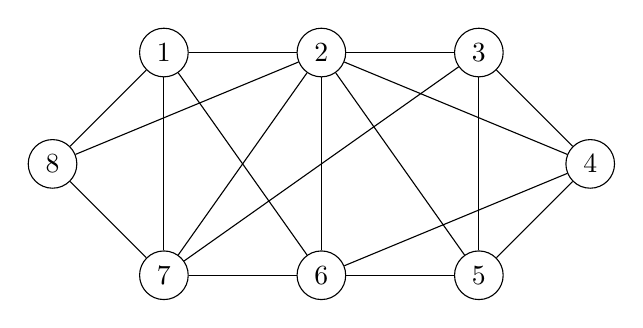
\begin{tikzpicture}[node distance=2cm]
			\node[circle, draw] (1)[] {$1$};
			\node[circle, draw] (2)[right of = 1] {$2$};
			\node[circle, draw] (3)[right of = 2] {$3$};
			\node[circle, draw] (4)[below right of = 3] {$4$};
			\node[circle, draw] (5)[below left of = 4] {$5$};
			\node[circle, draw] (6)[left of = 5] {$6$};
			\node[circle, draw] (7)[left of = 6] {$7$};
			\node[circle, draw] (8)[above left of = 7] {$8$};

			\path[every node/.style={font=\sffamily\small}]
				(1) edge (2)
				(2) edge (3)
				(3) edge (4)
				(4) edge (5)
				(5) edge (6)
				(6) edge (7)
				(7) edge (8)
				(8) edge (1)

				(1) edge (7)
				(2) edge (6)
				(2) edge (4)

				(1) edge[] (6)
				(8) edge[] (2)
				(7) edge[] (2)
				(7) edge[] (3)
				(3) edge[] (5)
				(5) edge[] (2)
				(6) edge[] (4)
			;
		\end{tikzpicture}
    \end{figure}

	A possible perfect elimination sequence for this 3-tree is given by $(8,1,7,2,6,5,3,4)$. By coloring the sequence in reverse order while preserving the $L(2,1)$-constraints we get the following color assignments.

    \begin{figure}[H]
		\centering

		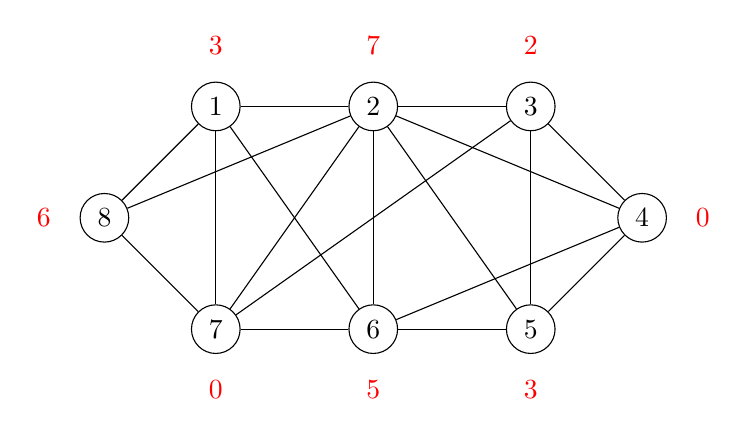
\begin{tikzpicture}[node distance=2cm]
			\node[circle, draw] (1)[] {$1$};
			\node[circle, draw] (2)[right of = 1] {$2$};
			\node[circle, draw] (3)[right of = 2] {$3$};
			\node[circle, draw] (4)[below right of = 3] {$4$};
			\node[circle, draw] (5)[below left of = 4] {$5$};
			\node[circle, draw] (6)[left of = 5] {$6$};
			\node[circle, draw] (7)[left of = 6] {$7$};
			\node[circle, draw] (8)[above left of = 7] {$8$};

			\node[color=red] (1a)[above of = 1, yshift=-35] {$3$};
			\node[color=red] (2a)[above of = 2, yshift=-35] {$7$};
			\node[color=red] (3a)[above of = 3, yshift=-35] {$2$};
			\node[color=red] (4a)[right of = 4, xshift=-35] {$0$};
			\node[color=red] (5a)[below of = 5, yshift=35] {$3$};
			\node[color=red] (6a)[below of = 6, yshift=35] {$5$};
			\node[color=red] (7a)[below of = 7, yshift=35] {$0$};
			\node[color=red] (8a)[left of = 8, xshift=35] {$6$};


			\path[every node/.style={font=\sffamily\small}]
				(1) edge (2)
				(2) edge (3)
				(3) edge (4)
				(4) edge (5)
				(5) edge (6)
				(6) edge (7)
				(7) edge (8)
				(8) edge (1)

				(1) edge (7)
				(2) edge (6)
				(2) edge (4)

				(1) edge[] (6)
				(8) edge[] (2)
				(7) edge[] (2)
				(7) edge[] (3)
				(3) edge[] (5)
				(5) edge[] (2)
				(6) edge[] (4)
			;
		\end{tikzpicture}

    \end{figure}

	\newpage

	We now prove that the algorithm always works with the following values.
	\begin{theorem}
		Given any graph $G$ of treewidth $k$, the Algorithm 1 finds:
		\begin{enumerate}
			\item An $L(2, 1)$-labeling using the set $\{0, \ldots, k\Delta + 2k\}$.
			\item An $L(1, 1)$-labeling using the set $\{0, \ldots, k\Delta\}$.
			\item An $L(0, 1)$-labeling using the set $\{0, \ldots, k\Delta-k\}$.
		\end{enumerate}
	\end{theorem}

	\begin{proof}
		Since the Algorithm 1 clearly produces an $L(p,q)$-labeling, it suffices to show that the largest colors claimed by the theorem are enough. Given a vertex $v_i$, where $1 \leq i \leq n$, we count the number of colors that are forbidden for $v_i$ when it gets colored. In particular, due to the $L(p,q)$ constraints,  can be one of three types of color forbidding nodes:
		\begin{enumerate}
			\item $\alpha$ already colored neighbors of $v_i$ in $G$.
			\item $\beta$ already colored vertices that are at distance two from $v_i$ in $G$ and that have a neighbor in common with $v_i$ which has yet to be colored.
			\item $\gamma$ already colored vertices that are at distance two from $v_i$ in $G$ and that have a neighbor in common with $v_i$ which has already been colored.
		\end{enumerate}

		By construction of the perfect elimination sequence on a $k$-tree, each vertex has at most $k$ neighbors in $H$ that come after it in the sequence. We will show that each of the three cases account for one of such at most $k$ neighbors, i.e. that $\alpha + \beta + \gamma$.
		
		Clearly, any type 1 vertex is one of such at most $k$ neighbors in $H$. Let $v_j$ be an already colored vertex at distance 2. If $v_j$ is a type 2 vertex, then we know that $h < i < j$ since the common neighbor $v_h$ has yet to be colored. Thus, by construction of the perfect elimination sequence, since $v_i$ and $v_j$ are adjacent to $v_h$ and they come after it in the sequence, they must be inside $v_h$'s neighbors that form a clique, concluding that $v_i$ and $v_j$ must be adjacent. Hence, $v_j$ must be one of $v_i$'s at most $k$ neighbors in $H$ that come after it.

		Suppose now that $v_j$ is a type 3 vertex. Since the common neighbor $v_h$ has already been colored, we know that $i < h, j$, meaning that $v_h$ must be one of the at most $k$ clique neighbors of $v_i$ in $H$. Each of these neighbors can have at most $\Delta-1$ already-colored adjacent nodes different from $v_i$, for a total of at most $\gamma(\Delta-1)$ vertices at distance 2 from $v_i$. Moreover, since $v_h$ is adjacent to $v_i$, it must be one of $v_i$'s at most $k$ neighbors in $H$ that come after it. This concludes that $\alpha + \beta + \gamma$.
		
		Let $x_{p,q}$ be the number of colors needed by Algorithm 1 to color $v_i$. Assume that $p = 2$ and $q = 1$. Each type 1 vertex forbids $3$ colors to $v_i$. In type 2 vertices, only the node $v_j$ has already been colored, implying that only $1$ color is forbidden to $v_i$. In type 3 vertices, instead, the node $v_h$ has already been colored and it can have at most $(\Delta-1)$ already-colored neighbors. We conclude that:
		\[x_{2,1} \leq 1+ 3\alpha + \beta + \gamma(\Delta-1) \leq 1+ 3k + k(\Delta-1) = 1+k\Delta + 2k\]

		When $p,q = 1$, each type 1 vertex forbids only $1$ color to $v_i$, concluding that:
		\[x_{1,1} \leq 1+ \alpha + \beta + \gamma(\Delta-1) \leq 1+3k + k(\Delta-1) = 1+k\Delta\]

		Finally, when $p = 0$ and $q = 1$ we can ignore type 1 vertices:
		\[x_{0,1} \leq 1 + \beta + \gamma(\Delta-1) \leq 1+3k + k(\Delta-1) = 1+k\Delta -k\]
	\end{proof}

	\begin{corollary}
		Given any graph $G$ of treewidth $k$ it holds that:
    	\[\lambda_{2,1} \leq k\Delta+2k \qquad\qquad \lambda_{1,1} \leq k\Delta \qquad\qquad \lambda_{0,1} \leq k\Delta-k\]
	\end{corollary}

	\section{Outerplanar graphs}

	We now consider outerplanar graphs. A graph is \textit{outerplanar} if it has a planar embedding such that all vertices touch the exterior face. Clearly, any outerplanar graph is a planar graph.

	\begin{figure}[H]
		\centering
		\begin{tabular}{ccc}
			\begin{tabular}{c}
				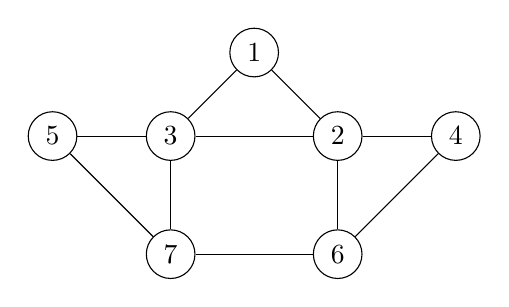
\begin{tikzpicture}[node distance=1.5cm]
					\node[circle, draw] (1)[] {$1$};
					\node[circle, draw] (2)[below right of = 1] {$2$};
					\node[circle, draw] (3)[below left of = 1] {$3$};
					\node[circle, draw] (4)[right of = 2] {$4$};
					\node[circle, draw] (5)[left of = 3] {$5$};
					\node[circle, draw] (6)[below of = 2] {$6$};
					\node[circle, draw] (7)[below of = 3] {$7$};

					\path[every node/.style={font=\sffamily\small}]
						(1) edge (2)
						(1) edge (3)
						(2) edge (4)
						(3) edge (5)
						(2) edge (6) 
						(3) edge (7)
						(6) edge (7)
						(5) edge (7)
						(4) edge (6)
						(2) edge (3)
					;
				\end{tikzpicture}
			\end{tabular}

			&\qquad&

			\begin{tabular}{c}
				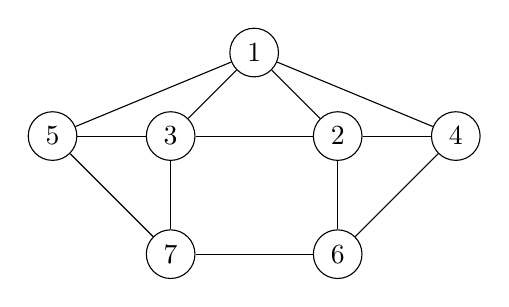
\begin{tikzpicture}[node distance=1.5cm]
					\node[circle, draw] (1)[] {$1$};
					\node[circle, draw] (2)[below right of = 1] {$2$};
					\node[circle, draw] (3)[below left of = 1] {$3$};
					\node[circle, draw] (4)[right of = 2] {$4$};
					\node[circle, draw] (5)[left of = 3] {$5$};
					\node[circle, draw] (6)[below of = 2] {$6$};
					\node[circle, draw] (7)[below of = 3] {$7$};

					\path[every node/.style={font=\sffamily\small}]
						(1) edge (2)
						(1) edge (3)
						(2) edge (4)
						(3) edge (5)
						(2) edge (6) 
						(3) edge (7)
						(6) edge (7)
						(5) edge (7)
						(4) edge (6)
						(2) edge (3)
						(1) edge (4)
						(1) edge (5)
					;
				\end{tikzpicture}
			\end{tabular}
		\end{tabular}
		\label{outerplanar}
		\caption{An outerplanar graph (left), a planar graph (right)}
    \end{figure}

	Upper bounds for this class of graphs are already known, in particular $\lambda_{2,1} \leq 2\Delta +2$ was shown in \cite{out_bound}. Using an algorithm similar to the previous one, we can improve this lower bound: we define a sequence of vertices and color them in reverse order. To define the sequence, the algorithm exploits the following lemma.

	\begin{lemma}
		\label{lemma_outer}
		If $G$ is an outerplanar graph then one of the two holds:
		\begin{itemize}
			\item There exists a vertex of degree at most one.
			\item There exists a vertex of degree at most two which
			has a neighbor of degree at most four.
		\end{itemize}
	\end{lemma}

	\begin{figure}[H]
		\begin{algorithmic}[1]
			\Function{algorithm 2}{$G$, $\lambda, p,q$}
				\State Let $H = G$
				\State Let $S = v_1, \ldots, v_n$
				\For{$i$ = $1, \ldots, n$}
					\State Let $u_i$ be a vertex that satisfies \Cref{lemma_outer}
					\If{$u_i$ has two neighbors $x,y$ that aren't adjacent in $H$}
						\State{Add the edge $(x,y)$ in $H$}
					\EndIf
					\State{Set $v_i = u_i$}
					\State{Remove $u_i$ from $H$}
				\EndFor
				\For{$i$ = $n, \ldots, 1$}
					\State{Color $v_i$ with the smallest available color in $\{0,\ldots, \lambda\}$ \\satisfying the $L(p,q)$-coloring constraints in $G$}
				\EndFor
			\EndFunction
		\end{algorithmic}

		\caption{Algorithm for $\lambda$-Coloring outerplanar graphs}
	\end{figure}

	In particular, we notice that, while computing the sequence $v_1, \ldots, v_n$, the graph obtained by removing $u_i$ and adding the edge $(x,y)$ is still outerplanar, hence the lemma can always be applied. Using a counting argument similar to the one used for the previous algorithm, we obtain the following.

	\begin{theorem}
		Given any outerplanar graph $G$, the Algorithm 2 finds:
		\begin{enumerate}
			\item An $L(2, 1)$-labeling using the set $\{0, \ldots, \Delta + 8\}$.
			\item An $L(1, 1)$-labeling using the set $\{0, \ldots, \Delta + 4\}$.
			\item An $L(0, 1)$-labeling using the set $\{0, \ldots, \Delta + 2\}$.
		\end{enumerate}
	\end{theorem}

	\begin{proof}
		First, we notice that in each iteration $H$ is always outerplanar thanks to the edge (added or already existing) that connects the two neighbors of the removed node.

		Assume that the sequence always picks a node $v_i$ with degree at most 2 who has a neighbor u of degree at most 4. Let $w$ be the other neighbor of $v_i$ (assuming it exists). We notice that $u$ and $w$ can have at most $3 + \Delta - 1$ at distance 2 from $v_i$ that have already been colored. Moreover, $u$ and $w$ can also be colored already. Let $x_{p,q}$ be the number of colors needed by Algorithm 2 to color $v_i$. We get that:
		\[\begin{split}
			x_{2,1} &\leq 1 + 3 \cdot 2 + (3+\Delta -1) = 1 + \Delta + 8 \\
			x_{1,1} &\leq 1 + 2 + (3+\Delta -1) = 1 + \Delta + 4 \\
			x_{0,1} &\leq 1 + (3+\Delta -1) = 1 + \Delta + 2
		\end{split}\]
	\end{proof}

	\begin{corollary}
		Given any outerplanar graph $G$ it holds that:
    	\[\lambda_{2,1} \leq \Delta+8 \qquad\qquad \lambda_{1,1} \leq \Delta+6 \qquad\qquad \lambda_{0,1} \leq \Delta+2\]
	\end{corollary}

	\section{Split graphs}

	We now move to the last class of graph, i.e. split graphs. A split graph is a graph $G$ whose node set can be partitioned into two sets $K$ and $S$ such that $K$ is a clique and $S$ is an independent set in $G$.

	\begin{figure}[H]
		\centering
		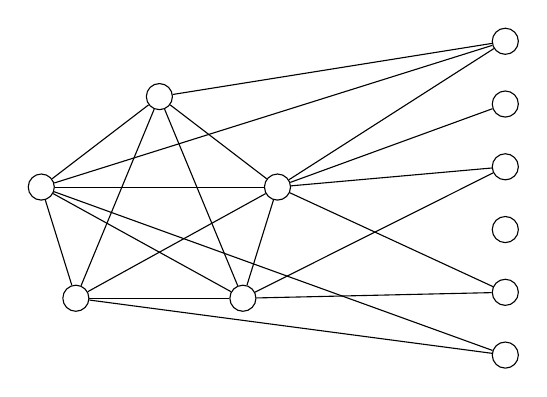
\begin{tikzpicture}[node distance=1.5cm]
			\node[] (1)[] {};
			\node[circle, draw] (2)[above of = 1, yshift=-10] {};
			\node[circle, draw] (3)[right of = 1] {};
			\node[circle, draw] (4)[below right of = 1, yshift=-10] {};
			\node[circle, draw] (5)[below left of = 1, yshift=-10] {};
			\node[circle, draw] (6)[left of = 1] {};

			\node[circle, draw] (7)[above of = 1, yshift=10, xshift=125] {};
			\node[circle, draw] (8)[below of = 7, yshift=20] {};
			\node[circle, draw] (9)[below of = 8, yshift=20] {};
			\node[circle, draw] (10)[below of = 9, yshift=20] {};
			\node[circle, draw] (11)[below of = 10, yshift=20] {};
			\node[circle, draw] (12)[below of = 11, yshift=20] {};

			\path[every node/.style={font=\sffamily\small}]
				(2) edge (3)
				(2) edge (4)
				(2) edge (5)
				(2) edge (6)
				(3) edge (4)
				(3) edge (5)
				(3) edge (6)
				(4) edge (5)
				(4) edge (6)
				(5) edge (6)

				(7) edge (2)
				(7) edge (3)
				(7) edge (6)
				(8) edge (3)
				(9) edge (3)
				(9) edge (4)
				(11) edge (3)
				(11) edge (4)
				(12) edge (5)
				(12) edge (6)
			;
		\end{tikzpicture}
		\label{split}
		\caption{A split graph}
    \end{figure}

	Using an algorithm similar to the two previously shown ones, we can also find upper bounds for this class of graphs (see \cite{main_article} for info on the third algorithm).

	\begin{corollary}
		Given any split graph $G$ it holds that:
    	\[\lambda_{2,1} \leq \frac{1}{2}\Delta^{1.5} + 2\Delta \qquad\qquad \lambda_{1,1} \leq \frac{1}{2}\Delta^{1.5} + \Delta \qquad\qquad \lambda_{0,1} \leq \frac{1}{2}\Delta^{1.5}\]
	\end{corollary}

	However, we won't focus on this third algorithm, as we are more interested in showing lower bounds for this class of graphs. In particular, we can show the following.

	\begin{theorem}
		For any $\Delta > 0$, there is a split graph with maximum degree $\Delta$ such that:
		\[\lambda_{2,1} \geq \lambda_{1,1} \geq \lambda_{0,1} \geq \frac{1}{2} \sqrt{\frac{2}{3}} \Delta^{1.5}\]
	\end{theorem}

	\begin{proof}
		Let $S$ be an independent set partitioned into $\sqrt{\frac{2}{3}\Delta}$ groups of $\frac{1}{3} \Delta$ nodes, for a total of $\frac{1}{2} \sqrt{\frac{2}{3}} \Delta^{1.5}$ nodes in $S$. We also notice that we have $\frac{\sqrt{\frac{2}{3}\Delta}\left (\sqrt{\frac{2}{3}\Delta}-1 \right )}{2} \leq \frac{1}{3}\Delta$ distinct pairs of groups in this partition. 

		Let $K$ be a clique of $\frac{1}{3}\Delta+1$ nodes. For each pair of groups, we take one unique node in the clique and make that node adjacent to each node in the two groups of the pair. Hence, each node in the clique now has at most $3 \cdot \frac{1}{3}\Delta = \Delta$ neighbors, making the graph a valid example. Moreover, we notice that this graph has diameter two and any pair of
		vertices in the independent set has distance exactly two. This means that we need at least one different color for each node in the independent set in order to satisfy the $L(0,1)$-constraints, meaning that we need at least $\frac{1}{2} \sqrt{\frac{2}{3}} \Delta^{1.5}$ nodes.
	\end{proof}


	\begin{figure}[H]
		\centering

		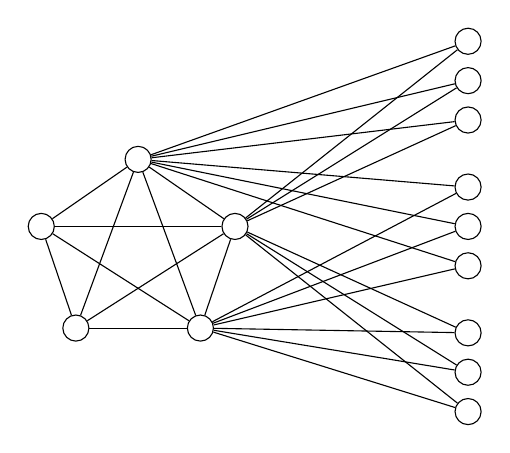
\begin{tikzpicture}[node distance=0.5cm]
			\node[circle, draw] (1)[] {};
			\node[circle, draw] (2)[below of = 1] {};
			\node[circle, draw] (3)[below of = 2] {};
			\node[circle, draw] (4)[below of = 3, yshift=-10] {};
			\node[circle, draw] (5)[below of = 4] {};
			\node[circle, draw] (6)[below of = 5] {};
			\node[circle, draw] (7)[below of = 6, yshift=-10] {};
			\node[circle, draw] (8)[below of = 7] {};
			\node[circle, draw] (14)[below of = 8] {};

			\node[circle, draw] (9)[left of = 5, xshift=-70] {};
			\node[circle, draw] (10)[above of = 9, xshift=-35, yshift=10] {};
			\node[circle, draw] (11)[below of = 10, xshift=-35, yshift=-10] {};
			\node[circle, draw] (12)[below of = 11, xshift=12.5, yshift=-22.5] {};
			\node[circle, draw] (13)[below of = 9, xshift=-12.5, yshift=-22.5] {};

			\path[every node/.style={font=\sffamily\small}]
				(9) edge (10)
				(9) edge (11)
				(9) edge (12)
				(9) edge (13)
				(10) edge (11)
				(10) edge (12)
				(10) edge (13)
				(11) edge (12)
				(11) edge (13)
				(12) edge (13)

				(9) edge (1)
				(9) edge (2)
				(9) edge (3)
				(9) edge (7)
				(9) edge (8)
				(9) edge (14)

				(10) edge[] (1)
				(10) edge[] (2)
				(10) edge[] (3)
				(10) edge[] (4)
				(10) edge[] (5)
				(10) edge[] (6)

				(13) edge[] (4)
				(13) edge[] (5)
				(13) edge[] (6)
				(13) edge[] (7)
				(13) edge[] (8)
				(13) edge[] (14)

			;
		\end{tikzpicture}

		\caption{The graph constructed by the proof with $\Delta = 10$}
	\end{figure}

	This lower bound is almost equal to the upper bound, especially in the $\lambda_{0,1}$ case. We also notice that, by definition, each split graph is also a chordal graph. This implies that the lower bounds of the previous theorem also hold for chordal graphs, and thus also for $k$-trees.


	\begin{corollary}
		For any $\Delta > 0$, there is a chordal graph with maximum degree $\Delta$ such that:
		\[\lambda_{2,1} \geq \lambda_{1,1} \geq \lambda_{0,1} \geq \frac{1}{2} \sqrt{\frac{2}{3}} \Delta^{1.5}\]
	\end{corollary}

	\newpage

    \printbibliography

\end{document}